\documentclass[tikz,border=4pt]{standalone}
\usepackage{amsmath}
\usetikzlibrary{arrows.meta,positioning,fit}
\definecolor{seionblue}{HTML}{0072B2}
\definecolor{seiongreen}{HTML}{009E73}
\definecolor{seionorange}{HTML}{E69F00}
\definecolor{seionred}{HTML}{D55E00}
\definecolor{seionpurple}{HTML}{CC79A7}
\definecolor{seiongray}{HTML}{6B7280}
\tikzset{
  item/.style={draw,rounded corners=2pt,align=center,minimum width=27mm,minimum height=9mm,fill=white,line width=.85pt},
  proof/.style={item,draw=seiongreen},
  upper/.style={item,draw=seionblue},
  lower/.style={item,draw=seionorange},
  empirical/.style={item,draw=seionpurple},
  blocked/.style={item,draw=seionred,fill=seionred!5},
  edge/.style={-{Stealth[length=1.8mm]},line width=.75pt,seiongray}
}
\begin{document}
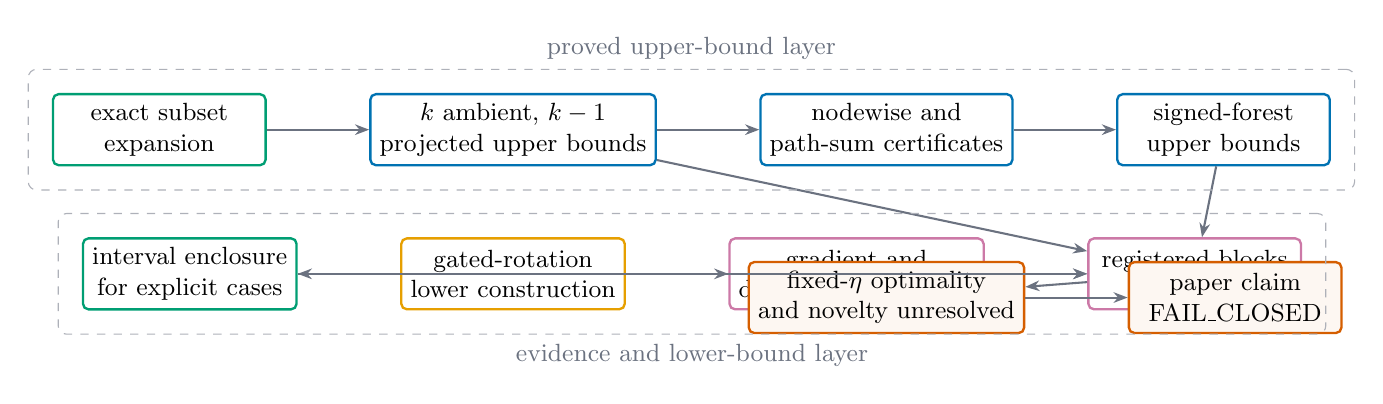
\begin{tikzpicture}[font=\small,node distance=9mm and 13mm]
  \node[proof] (exact) {exact subset\\expansion};
  \node[upper,right=of exact] (hom) {$k$ ambient, $k-1$\\projected upper bounds};
  \node[upper,right=of hom] (nodewise) {nodewise and\\path-sum certificates};
  \node[upper,right=of nodewise] (forest) {signed-forest\\upper bounds};

  \node[lower,below=of hom] (construction) {gated-rotation\\lower construction};
  \node[empirical,right=of construction] (search) {gradient and\\derivative-free search};
  \node[proof,left=of construction] (interval) {interval enclosure\\for explicit cases};
  \node[empirical,right=of search] (matrix) {registered blocks\\A--I};

  \node[blocked,below=12mm of nodewise] (novelty) {fixed-$\eta$ optimality\\and novelty unresolved};
  \node[blocked,right=of novelty] (release) {paper claim\\FAIL\_CLOSED};

  \draw[edge] (exact) -- (hom);
  \draw[edge] (hom) -- (nodewise);
  \draw[edge] (nodewise) -- (forest);
  \draw[edge] (construction) -- (interval);
  \draw[edge] (construction) -- (search);
  \draw[edge] (search) -- (matrix);
  \draw[edge] (interval) -- (matrix);
  \draw[edge] (hom) -- (matrix);
  \draw[edge] (forest) -- (matrix);
  \draw[edge] (matrix) -- (novelty);
  \draw[edge] (novelty) -- (release);

  \node[draw=seiongray!55,dashed,rounded corners=3pt,fit=(exact)(hom)(nodewise)(forest),inner sep=3mm,label={[seiongray]above:proved upper-bound layer}] {};
  \node[draw=seiongray!55,dashed,rounded corners=3pt,fit=(interval)(construction)(search)(matrix),inner sep=3mm,label={[seiongray]below:evidence and lower-bound layer}] {};
\end{tikzpicture}
\end{document}
